% Phantom + Hab + Mars

\subsection{Phantom in Mars Habitat Module}
The purpose of this calculation was to demonstrate the ability to simulate a detailed
human phantom inside a habitat module in the radiation environment that exists on the
surface of Mars.  Some of the challenges included finding a high fidelity human phantom
suitable for radiation transport, composing the full geometry from components generated
by different methods, and accurately simulating the GCR spectrum and applying it such
that a fair number of particles would reach the regions of interest. Proof of this
capability is a necessary first step in the ultimate goal of calculating cancer risk
to astronauts in future Mars missions.

\subsection*{Geometry}
The human phantom geometry was generated by a medical physics group at the University of Florida.
First, a voxel model of the phantom was created from CT scan data.  The voxel model
was used to generate a Wavefront OBJ file and \texttt{ ReadOBJ} was then used to convert
the OBJ file to an HDF5 file.  

A CAD model of the habitat module was created by NASA and the ACIS file was imported 
into Trelis.  The DAGMC Trelis plugin was used to export a faceted version of the file.

As a first approximation, Mars was represented by a 1200 m x 1200 m x 10 m block of regolith.
The CAD model of the planet was created with Trelis and the faceted,
file was exported.  In the future, it could be found that topological features of
the planet make a significant difference in dose received by the human inside the 
habitat module.  In this case, a more detailed model of the planet will need to be used.

In this particular calculation, the atmosphere was not explicitly modeled by CAD geometry
surfaces due to the complicated boolean subtraction of surfaces that would need to occur
between the atmosphere and the habitat module.  Instead, the atmosphere was accounted 
for by giving the implicit compliment the composition and density of the atmospheric layer
closest to the surface of Mars.

\subsection*{Workflow}
HDF5 files of the phantom, habitat, and regolith were combined into a single geometry file
using the \texttt{combine\_geoms} tool.  The material compositions given in Appendix \ref{App:A1}
were used to generate a material library using the PyNE Material class.  Each object in
the geometry was tagged with a material.  The materials and tallies were then applied to the
geometry file via \texttt{uwuw\_preproc}.  Specifically, a NASA/CancerRisk tally was applied 
to all phantom objects that have the tally tag. \texttt{Mainfludag} was then used to generate the 
materials and cancer-risk scoring sections of the FLUKA input file.  Global mesh scoring 
for total energy deposition was also added to the input file.  The source used was the 
full GCR spectrum as detailed in previous sections.  


\subsection*{Results}

For proof of concept, a short \texttt{FluDAG}
calculation with 1e4 histories was run on a desktop machine.  Because so few histories 
were run, the cancer risk scoring in each phantom region did not yield any useful results.  
Many more histories will need to be run with the use of a computing cluster in order to 
achieve statistically accurate results.  The results from the global mesh scoring of 
energy deposition are shown below.  This successfully demonstrates the ability of a problem
of this scale to be run. 
 
%Figure~\ref{fig:results_fig} which is shown below.

\begin{figure}
 % Width = width of figure, {/path/to/figure.(png,pdf,jpg)}
 \begin{centering}
 \centering
 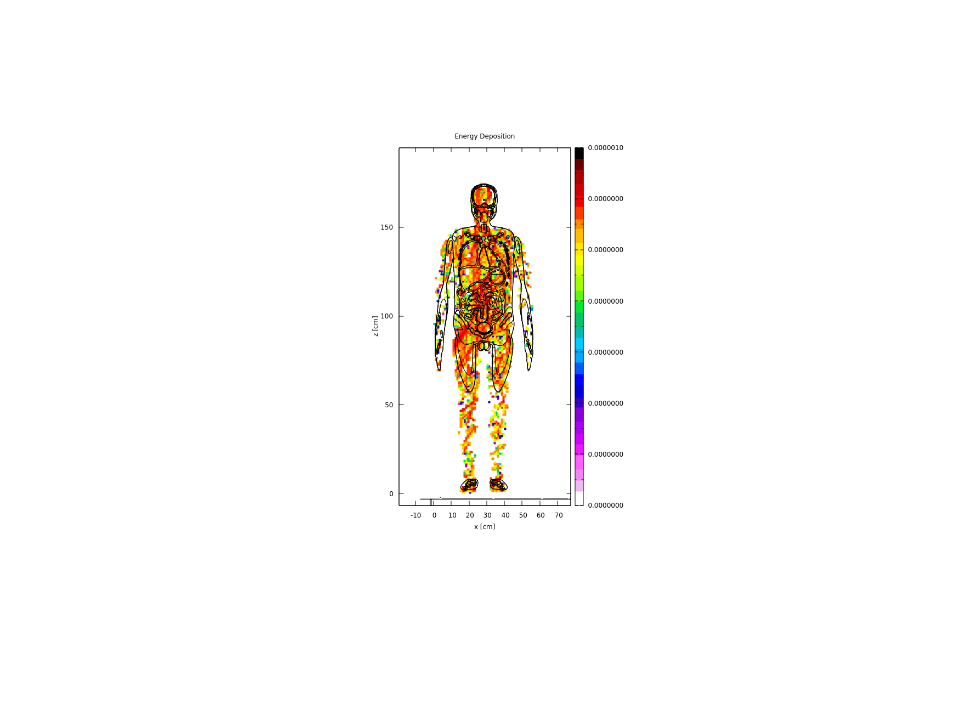
\includegraphics[width=\paperwidth]{../figs/phantom_ed.png}
 \caption{Energy deposition in phantom}
% \label{fig:results_fig}
 \end{centering}
\end{figure}
